% Ubah judul dan label berikut sesuai dengan yang diinginkan.
\section{Desain dan Implementasi}
\label{sec:desaindanimplementasi}

\begin{enumerate}[label=\Alph*.]
    \item Diagram Blok Sistem
    \label{subsec:diagrambloksistem}

    \hspace*{1em} Sistem yang telah dirancang memiliki beberapa komponen utama, yaitu bagian sensor, bagian kontrol, bagian sistem mekanik, dan bagian \textit{motion data}. 

    \begin{figure} [h] \centering
        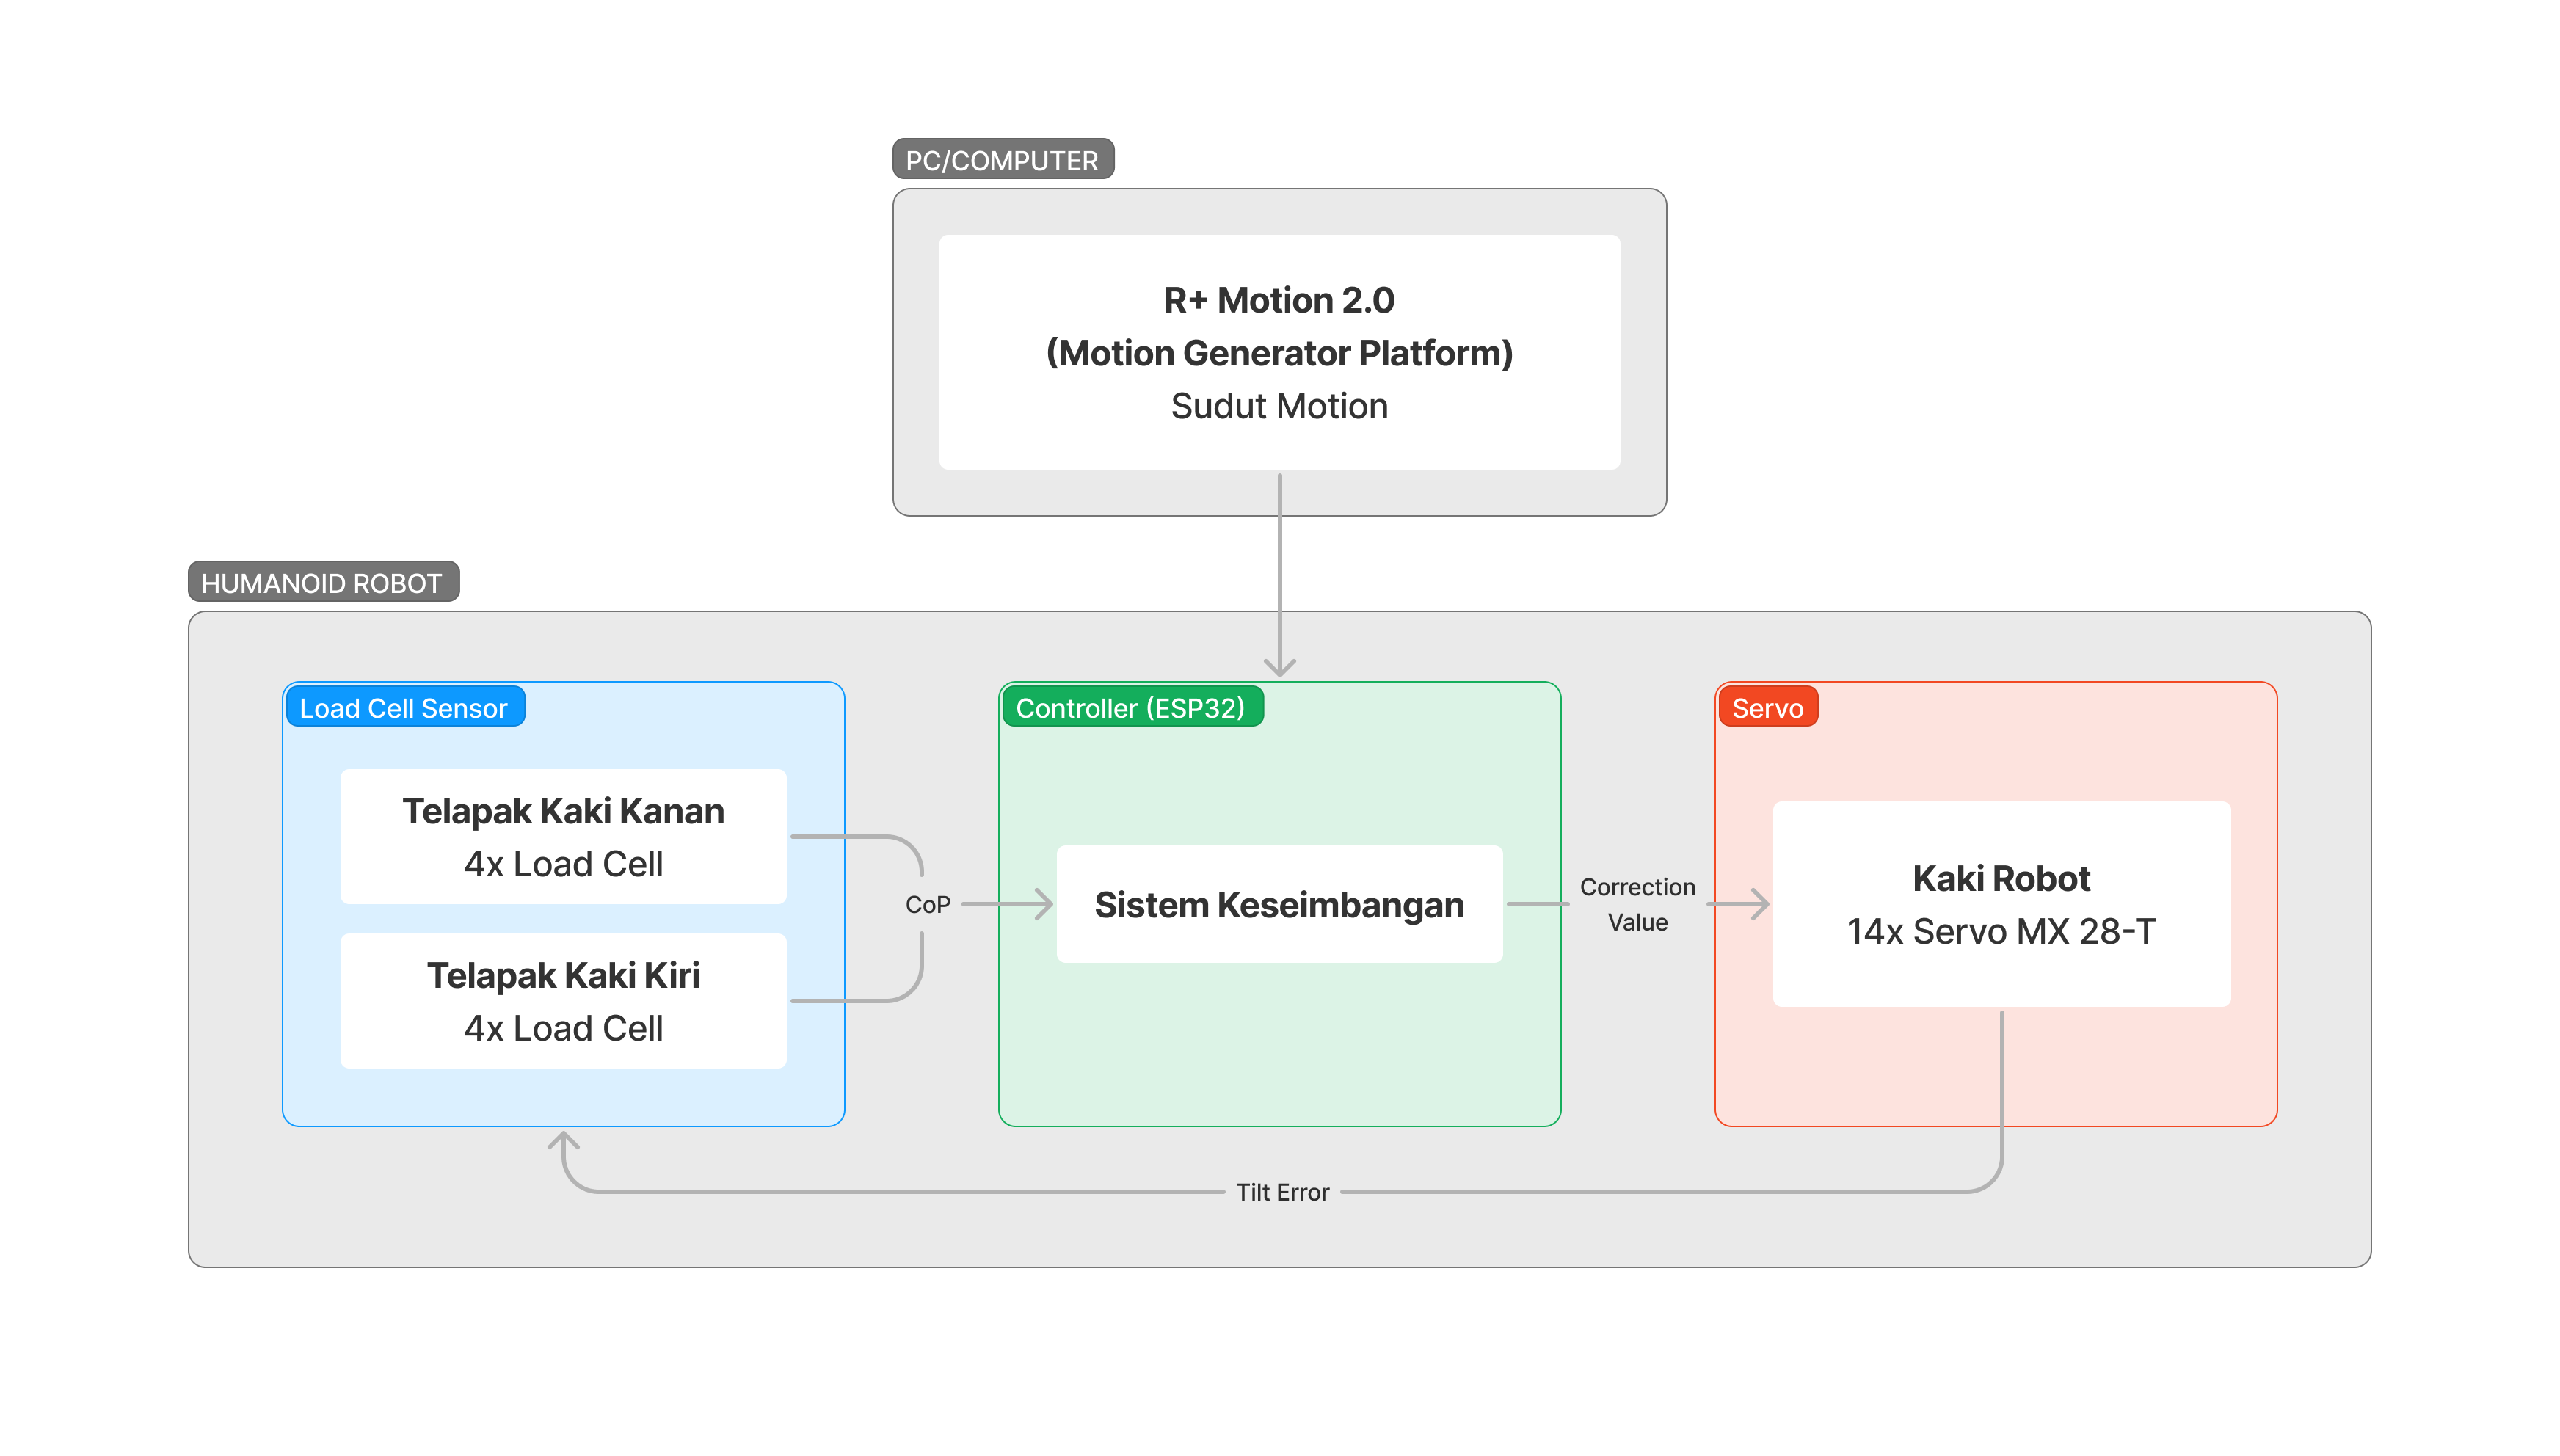
\includegraphics[width=0.45\textwidth]{gambar/Diagram_Sistem.png}
        \caption{Diagram Sistem Secara Keseluruhan}
        \label{fig:Diagram_Sistem}
    \end{figure}
    
    \hspace*{1em} Bagian sensor mencakup \emph{load cell} yang dipasang pada setiap telapak kaki robot. \emph{Load cell} ini berfungsi untuk mendeteksi beban atau tekanan pada kaki robot, memberikan informasi real-time yang diperlukan untuk menjaga keseimbangan robot. Bagian kontrol melibatkan mikrokontroler yang bertanggung jawab untuk mengolah data dari sensor dan mengontrol gerakan robot. Bagian sistem mekanik mencakup kerangka robot yang terdiri dari berbagai servo yang digunakan untuk menggerakkan robot. Bagian \textit{motion data} menyimpan gerakan yang telah dirancang sebelumnya dalam sistem file mikrokontroler. Data ini terdiri dari beberapa frame yang berisi array target posisi untuk setiap servo beserta waktu yang diperlukan untuk mencapai posisi tersebut. Diagram sistem dapat dilihat pada Gambar \ref{fig:Diagram_Sistem}.
    
    \item Sistem Mekanik
    \label{subsec:sistemmekanik}

    \hspace*{1em} Desain tubuh robot humanoid ini mencakup 29 derajat kebebasan. Tubuh bagian atas menggunakan 15 servo tipe XL-320, sedangkan tubuh bagian bawah menggunakan 14 servo tipe MX-28. Rincian desain, ukuran, dan penamaan ID servo pada robot dapat dilihat pada Gambar \ref{fig:Desain_Mekanik}. 

    \begin{figure} [h] \centering
      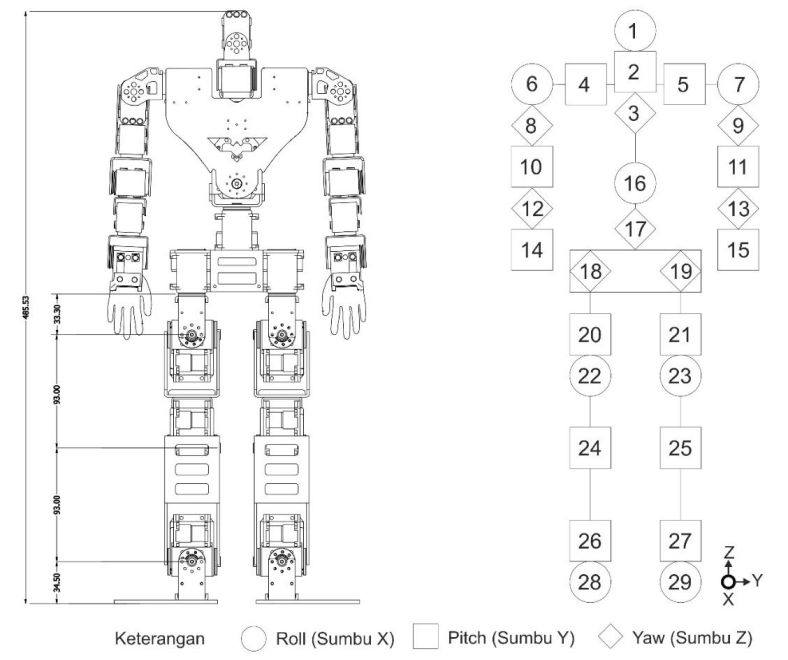
\includegraphics[width=0.35\textwidth]{gambar/Desain_Mekanik.png}
      \caption{Desain Mekanik Robot dan Penamaan ID Servo}
      \label{fig:Desain_Mekanik}
    \end{figure}

    \item Sistem Elektronik
    \label{subsec:sistemelektronik}

    \hspace*{1em} Sistem perangkat keras (hardware) dalam penelitian ini dijelaskan melalui diagram blok yang ditunjukkan pada Gambar \ref{fig:Diagram_Elektronik}. Sistem ini menggunakan sistem tertanam yang terdiri dari mikrokontroler ESP32 dan ESP32-C3. Sistem tertanam dipilih karena robot yang dikembangkan dalam penelitian ini merupakan pengembangan dari penelitian sebelumnya yang dilakukan oleh Fahd (2018)\cite{fahd}. 

    \begin{figure} [h] \centering
      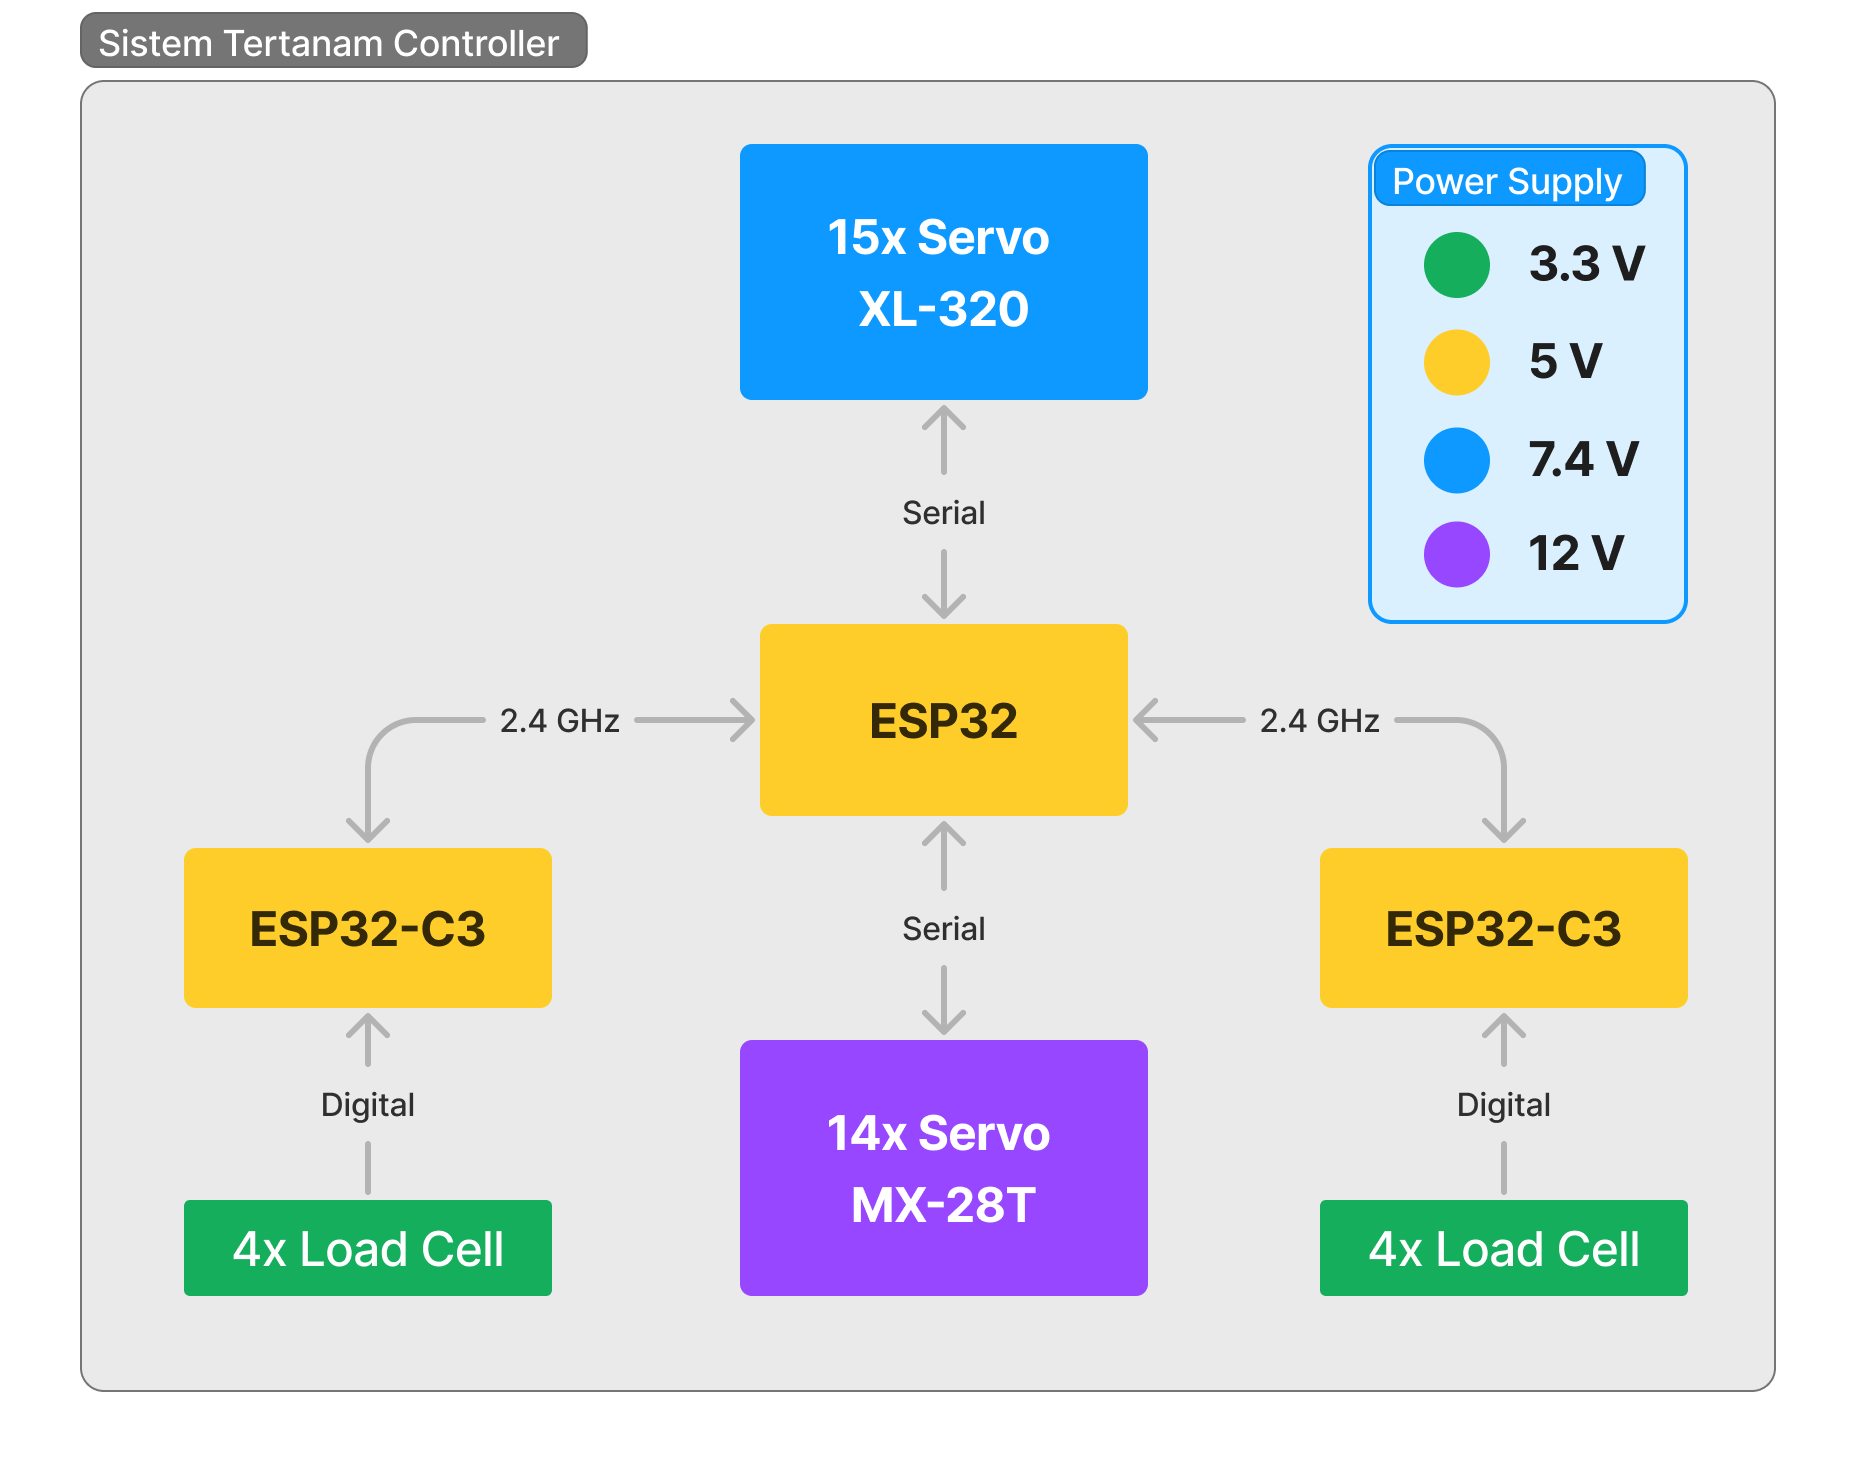
\includegraphics[width=0.4\textwidth]{gambar/Diagram_Elektronik.png}
      \caption{Diagram Elektronik dan Komunikasi Antar Komponen}
      \label{fig:Diagram_Elektronik}
    \end{figure}

    \hspace*{1em} ESP32-C3, digunakan untuk pengambilan data dari load cell dan mengirimkannya ke ESP32. ESP32-C3 memiliki kemampuan Wi-Fi yang sama dengan ESP32, sehingga memungkinkan komunikasi nirkabel antara dua mikrokontroler. ESP32-C3 juga memiliki dimensi yang lebih kecil, sehingga lebih mudah ditempatkan pada kaki robot.

    \item Desain Telapak Kaki Robot
    \label{subsec:desainsistemloadcell}

    \hspace*{1em} Setiap telapak kaki robot dilengkapi dengan 4 \emph{load cell} yang terpasang di ujung-ujung kaki. Masing-masing \emph{load cell} mendeteksi tekanan, sehingga memungkinkan sistem untuk menentukan posisi pusat tekanan pada telapak kaki robot. Desain telapak kaki robot dapat dilihat pada Gambar \ref{fig:Desain_Kaki}.
    
    \begin{figure} [h] \centering
      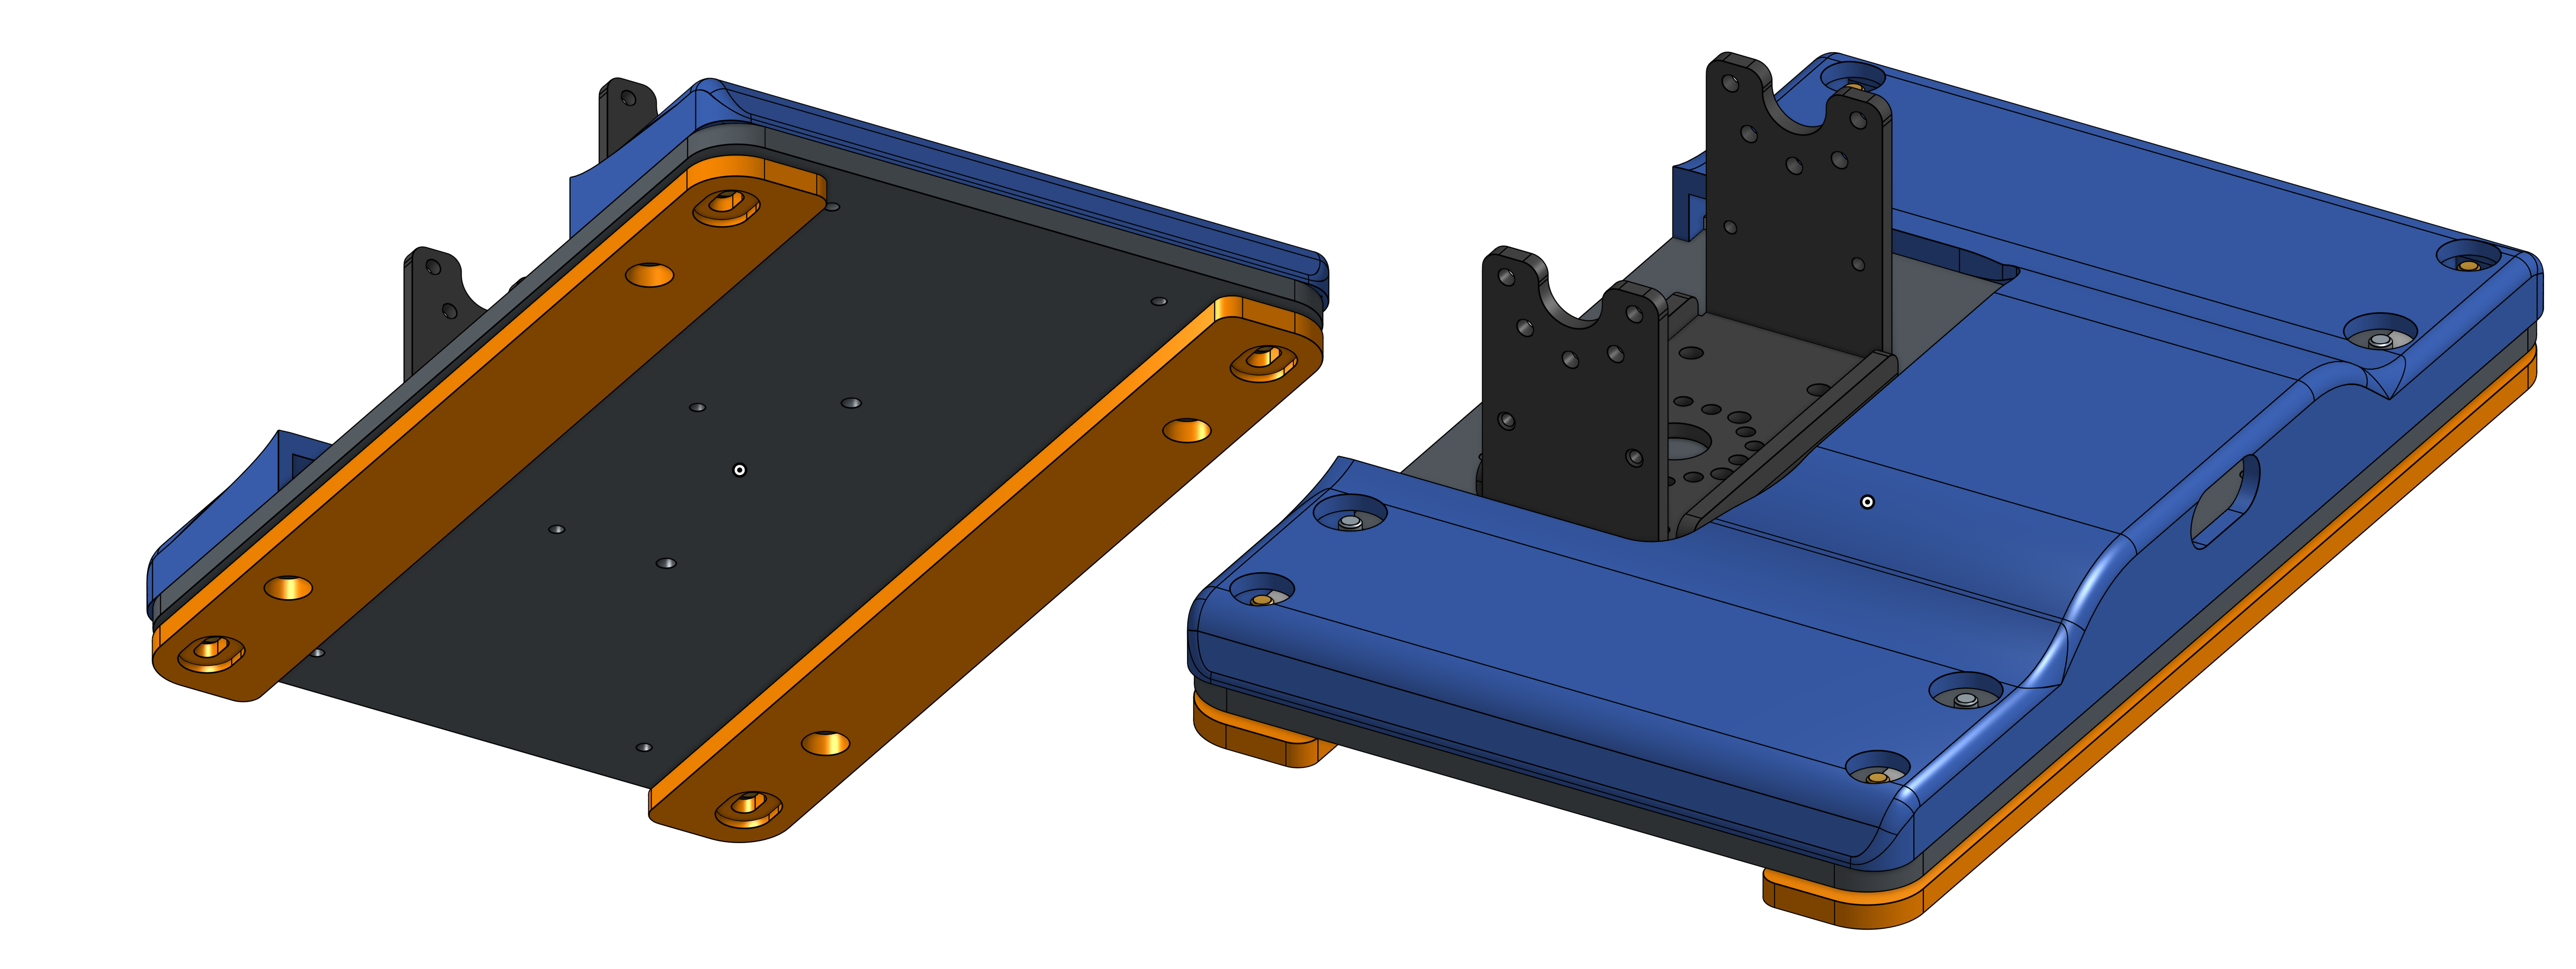
\includegraphics[width=0.4\textwidth]{gambar/Desain_Kaki.png}
      \caption{Desain Telapak Kaki Robot secara Keseluruhan}
      \label{fig:Desain_Kaki}
    \end{figure}

    \hspace*{1em} Pada Gambar \ref{fig:Desain_Kaki}, terlihat bahwa setiap \emph{load cell} ditempatkan pada ujung kaki robot. \emph{Load cell} tersebut terhubung ke mikrokontroler yang terletak di dalam kaki robot. Pada bagian elektronik, telah diberikan penutup berupa \textit{closure} yang terbuat dari 3D print untuk melindungi komponen dari kerusakan. Pada bagian mekanis, sensor \emph{load cell} dilengkapi dengan \textit{pad} yang berfungsi sebagai penekan sensor \emph{load cell} ke permukaan dan juga anti slip agar tidak mudah tergelincir.  

    \item Perhitungan Pusat Tekanan terhadap Robot
    \label{subsec:perhitunganpusattekanan}

    \hspace*{1em} Tekanan pada masing-masing load cell dijumlah dengan persamaan \ref{eq:Total_Force}. Hasil dari penjumlahan tersebut kemudian digunakan untuk menghitung posisi pusat tekanan pada sumbu x dan y dengan persamaan \ref{eq:COP_X} dan \ref{eq:COP_Y}. Pada posisi seimbang, posisi pusat tekanan akan berada pada titik (0,0) yang berada di tengah-tengah telapak kaki. Pusat tekanan tersebut dihitung dengan menjumlahkan tekanan terhadap titik pusat tekanan pada telapak kaki robot. Rentang nilai pusat tekanan pada telapak kaki robot adalah -1 hingga 1. Hasil dari perhitungan pusat tekanan tersebut kemudian dikirimkan ke mikrokontroler utama yang akan mengontrol gerakan robot. 

    \begin{equation}
      F_{\mathrm{total}} = F_1 + F_2 + F_3 + F_4
      \label{eq:Total_Force}
    \end{equation}

    \begin{equation}
      X_{\mathrm{cop}} = \frac{- F_1 + F_2 - F_3 + F_4}{F_{\mathrm{total}}}
      \label{eq:COP_X}
    \end{equation}

    \begin{equation}
      Y_{\mathrm{cop}} = \frac{F_1 + F_2 - F_3 - F_4}{F_{\mathrm{total}}}
      \label{eq:COP_Y}
    \end{equation}

    \item Algoritma Program Pemanggilan \textit{Motion}
    \label{subsec:algoritmamotion}

    \hspace*{1em} Sebelum robot dijalankan, program yang juga berisi data motion yang sudah dibuat sebelumnya diunggah ke dalam memori non-volatile pada  mikrokontroler. Motion yang diunggah berisi data untuk servo motor bagian atas dan bawah robot. Selanjutnya, robot dijalankan dan dimasukan input berupa index motion. Tiap index motion memiliki beberapa frame berdasarkan data motion yang telah diupload. Kemudian robot akan menjalankan gerakan satu persatu berdasarkan frame dari index motion yang dimasukkan.

    \begin{figure} [h]
      \centering
      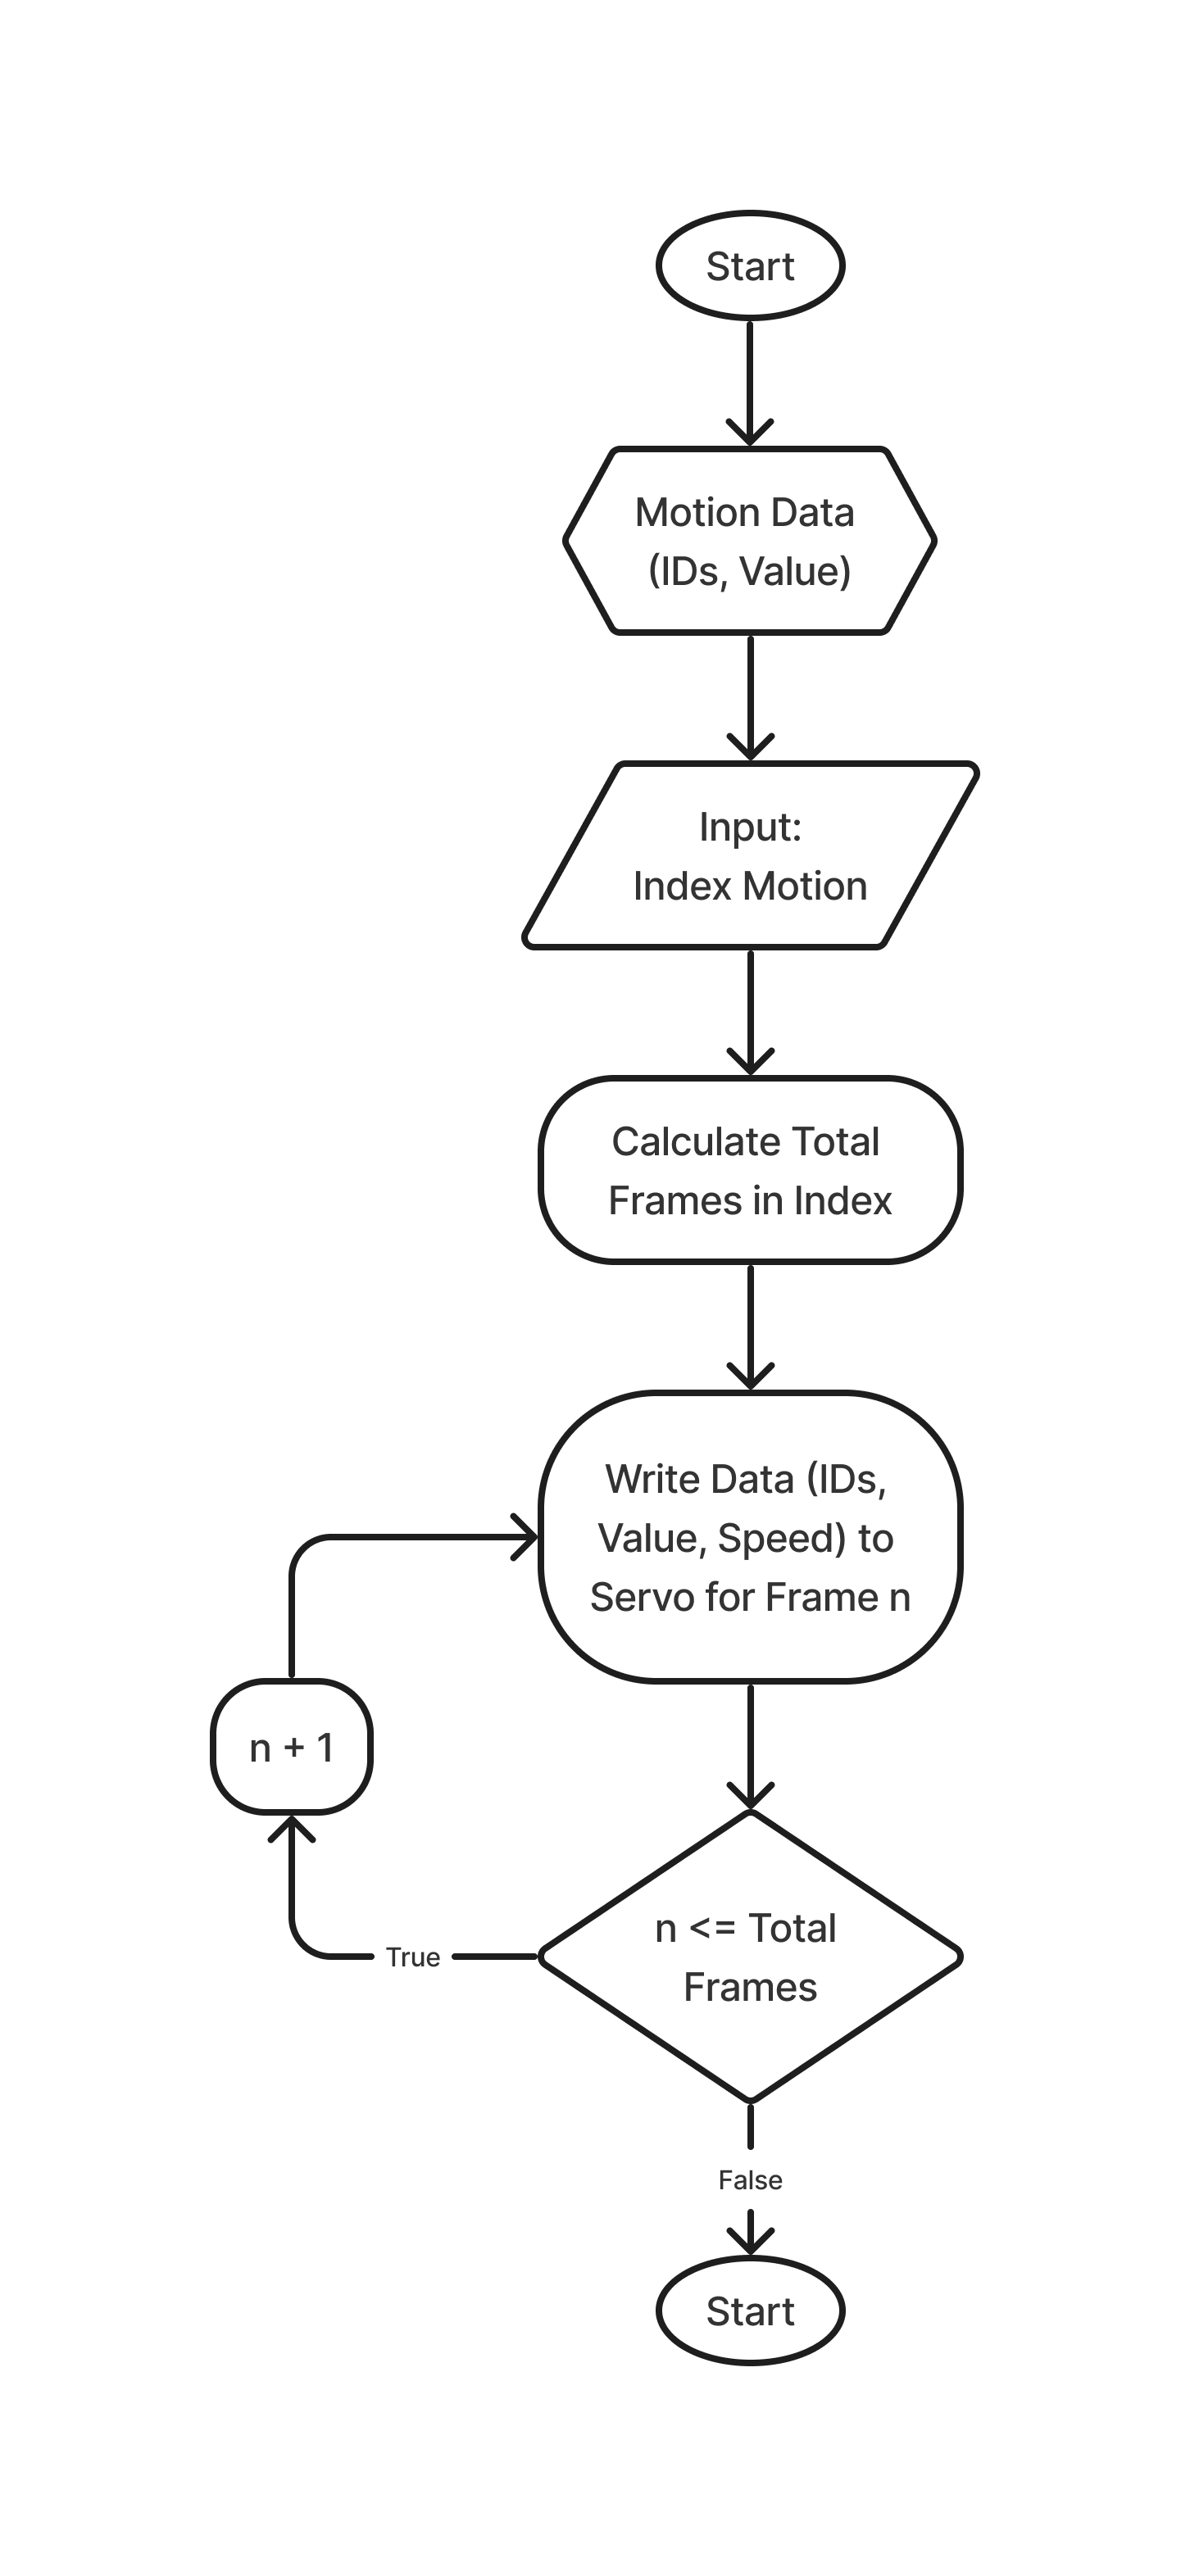
\includegraphics[width=0.3\textwidth]{gambar/flowchart_play_index.png}
      \caption{Diagram Alir Program Berjalan}
      \label{fig:Algoritma_Berjalan}
    \end{figure}

    \item Algoritma Kontrol PID
    \label{subsec:algoritmakontrolpid}

    \hspace*{1em} Pada penelitian ini, terdapat dua kontrol PID yang digunakan, yaitu kontrol PID Pitch dan kontrol PID Roll. Pada kontrol PID Pitch, input berupa nilai posisi pusat tekanan pada sumbu Y. Sedangkan pada kontrol PID Roll, input berupa nilai posisi pusat tekanan pada sumbu X. Untuk setpoint kontrol PID Pitch dan Roll, digunakan nilai yang sudah ditemukan pada pengambilan data input pusat tekanan sebelumnya. Nilai error diperoleh dari selisih antara posisi pusat tekanan saat ini dengan setpoint seperti pada Persamaan \ref{eq:Error_PID} dan koreksi PID dihitung dengan Persamaan \ref{eq:Koreksi_PID}.

    \begin{equation}
      \mathrm{e} = COP_{\mathrm{error}} = COP_{\mathrm{set}} - COP_{\mathrm{input}}
      \label{eq:Error_PID}
    \end{equation}

    \begin{equation}
      \mathrm{Koreksi} = \mathrm{Kp} \cdot \mathrm{e} + \mathrm{Ki} \cdot \int \mathrm{e} + \mathrm{Kd} \cdot \frac{\mathrm{de}}{\mathrm{dt}}
      \label{eq:Koreksi_PID}
    \end{equation}

    \item Servo Settings as Compensation
    \label{subsec:servosettings}

    \hspace*{1em} The servos used are located at the \textit{hip adduction} and \textit{ankle} because these two parts have a significant impact on the robot's posture stability when standing on one leg. The hip servo functions to control the upper part of the robot, while the ankle servo controls the movement of the foot. By precisely adjusting the servo angles, the robot can make the necessary adjustments to maintain balance when moving or standing on uneven surfaces.

    \begin{figure} [h] \centering
      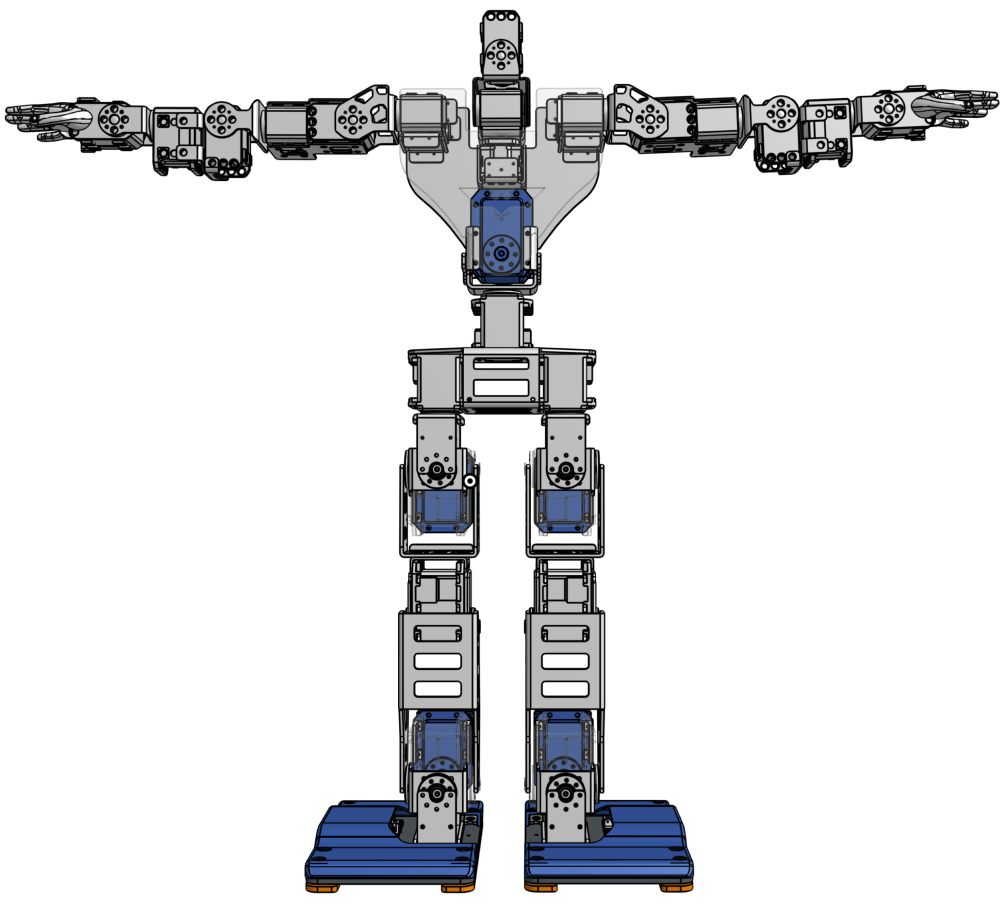
\includegraphics[width=0.4\textwidth]{gambar/controlled_servo.png}
      \caption{Servo Settings as Compensation}
      \label{fig:Controlled_Servo}
    \end{figure}

    \hspace*{1em} In this research, five servos are used to control the roll movement, consisting of two servos on each ankle, one servo on the torso, and two servos on each hip adduction. The servo settings as compensation can be seen in Figure \ref{fig:Controlled_Servo}, indicated by the blue-colored servos.
\end{enumerate}